\chapter{\textit{FrontEnd}}
Di seguito viene illustrato la parte di \textit{FrontEnd} del progetto. Verranno illustrate le principali funzionalità sviluppate ed alcuni dettagli implementativi.

\section{\textit{Home Page}}
    \begin{figure}[H]
        \centering
        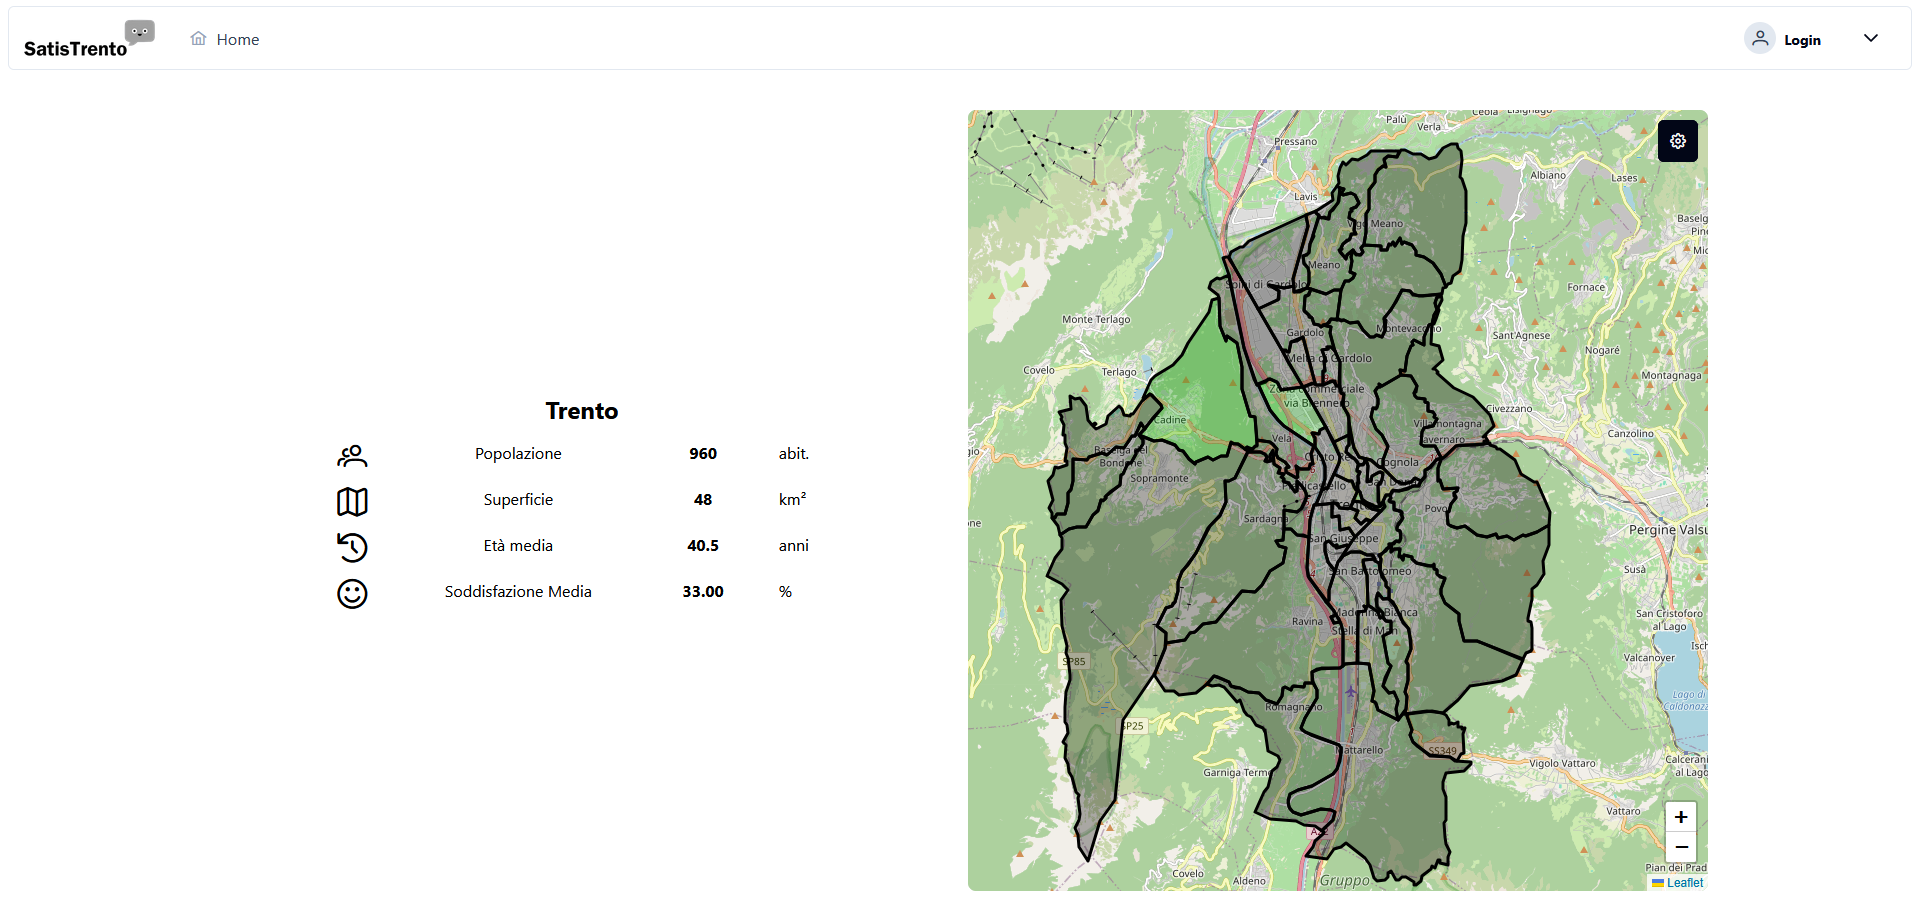
\includegraphics[width=0.8\textwidth]{frontend/home.png}
        \caption{\textit{Home Page} per utenti non loggati}
        \label{fig:frontend-home}
    \end{figure}
    Nella Figura \Ref{fig:frontend-home} è possibile vedere la \textit{Home Page} della \textit{web-app}. Come da specifiche descritte nei documenti precedenti questa presenta: i dati generali relativi all'intero comune, la mappa interattiva, tematica sulla base della soddisfazione media e suddivisa per quartieri. Nell'angolo in alto a destra della mappa è presente un pulsante per aprire il menù delle impostazioni per passare da ``quartieri'' a ``circoscrizioni'' e viceversa. Inoltre, nell'angolo superiore destro della pagina è presente un pulsante per accedere alla pagina di \textit{login}.
    
    \subsubsection{Dettaglio menù impostazioni}
        \begin{figure}[H]
            \centering
            
\includegraphics[width=0.3\textwidth]{frontend/opzioni_quart_circ.png}
            \caption{Menù impostazioni}
            \label{fig:frontend-settings}
        \end{figure}
        Come precedentemente descritto, il menù delle impostazioni sopra raffigurato, chiudibile premendo la ``X'', permette di passare da una visualizzazione dei dati per quartieri ad una per circoscrizioni e viceversa. La figura sopra è relativa a tutte le tipologie di utenti ad eccezione degli utenti con ruolo ``analista''.
\newpage
    \subsubsection{Selezione di un ``quartiere''/``circoscrizione''}
        \begin{figure}[H]
            \centering
            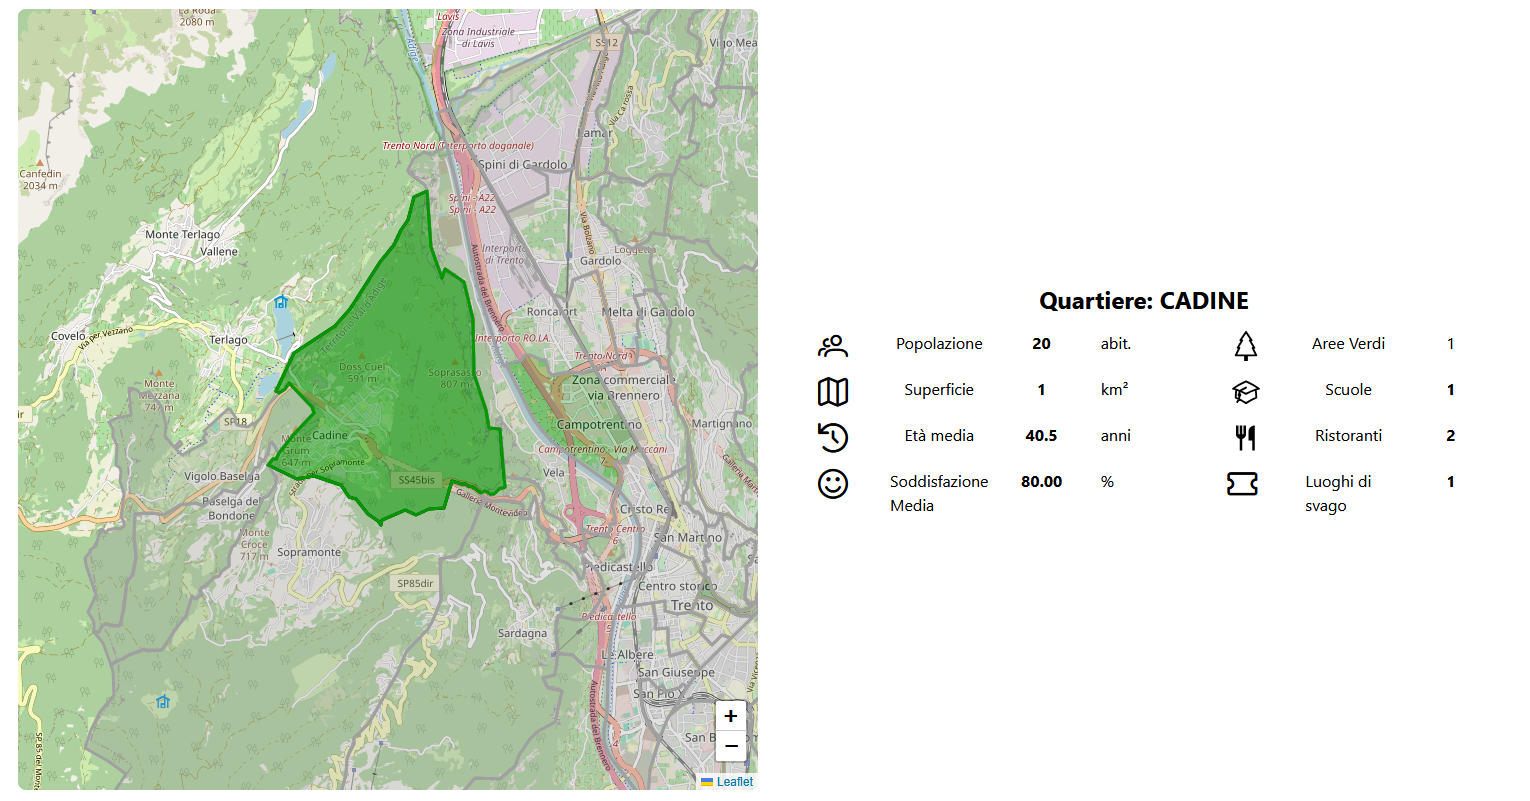
\includegraphics[width=0.8\textwidth]{frontend/quartiere_selezionato.png}
            \caption{Selezione di un ``quartiere''/``circoscrizione''}
            \label{fig:frontend-quartiere}
        \end{figure}
        Notiamo dalla Figura \Ref{fig:frontend-quartiere} come la selezione di un ``quartiere'' o ``circoscrizione'' avvenga tramite un click sulla mappa. Una volta selezionato un ``quartiere'' o ``circoscrizione'' verranno visualizzati degli ulteriori informazioni più specifiche riguardanti il ``quartiere'' o la ``circoscrizione'' selezionata. Inoltre il ``quartiere'' o la ``circoscrizione'' selezionata verrà evidenziata sulla mappa oscurano gli altri ``quartieri'' o le altre ``circoscrizioni'', inoltre la mappa avrà il suo centro sul centro del quartiere ed avrà uno zoom adeguato per visualizzare il ``quartiere'' o la ``circoscrizione'' selezionata nella sua interezza. Da questa schermata è possibile tornare alla visualizzazione generale ri-selezionando il ``quartiere'' o la ``circoscrizione'' selezionata oppure è possibile cambiare ``quartiere'' o ``circoscrizione'' selezionando un altro ``quartiere'' o ``circoscrizione'' dalla mappa.
\section{\textit{Login}}
    \begin{figure}[H]
        \centering
        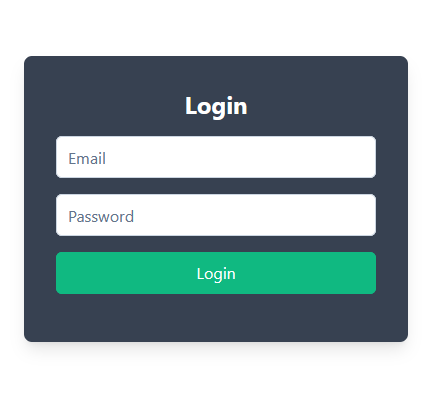
\includegraphics[width=0.4\textwidth]{frontend/dettaglio_login.png}
        \caption{Dettaglio pagina di \textit{login}}
        \label{fig:frontend-login}
    \end{figure}
    Nella Figura \Ref{fig:frontend-login} è possibile vedere il dettaglio della pagina di \textit{login}. Da questa pagina tutti gli utenti in possesso di credenziali valide possono accedere. \newpage
        \subsubsection{Messaggio di errore}
        \begin{figure}[H]
            \centering
            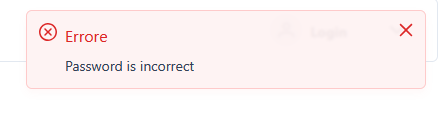
\includegraphics[width=0.4\textwidth]{frontend/dettaglio_errore_login.png}
            \caption{Messaggio di errore}
            \label{fig:frontend-login-error}
        \end{figure}
        Nella Figura \Ref{fig:frontend-login-error} è possibile vedere come si presenta il messaggio di errore in caso di credenziali errate. Questo viene visualizzato per $5$ secondi in caso di credenziali errate o altro errore.\newline
        Si noti come il presente ``formato'' di \textit{feedback} per i messaggi di errori sia stato implementato per tutte le pagine della \textit{web-app} in caso di un qualsiasi errore, viene difatti mostrato il titolo dell'errore con l'azione che non è stata possibile effettuare ed una descrizione più dettagliata del perché non è stato possibile effettuare l'azione richiesta.
        \subsubsection{Messaggio di login effettuato}
        \begin{figure}[H]
            \centering
            
\includegraphics[width=0.4\textwidth]{frontend/dettaglio_messaggio_login.png}
            \caption{Messaggio di login effettuato}
            \label{fig:frontend-login-success}
        \end{figure}
        Nella Figura \Ref{fig:frontend-login-success} è possibile vedere come si presenta il messaggio di login effettuato con successo. Questo viene visualizzato per $3$ secondi in caso di login effettuato con successo.\newline
        Si noti come il presente ``formato'' di \textit{feedback} sia stato implementato per tutte le pagine della \textit{web-app} in caso di un qualsiasi errore, viene difatti mostrato la scritta ``successo'', o altra equivalente, ed una breve descrizione di cosa è stato effettuato con successo.
\section{funzionalità Analista}
    Nella seguente sezione verranno illustrate le funzionalità disponibili per gli utenti con ruolo ``analista''. Questi utenti hanno accesso a funzionalità specifiche per la loro mansione e non disponibili agli altri utenti.
    \begin{figure}[H]
        \centering
        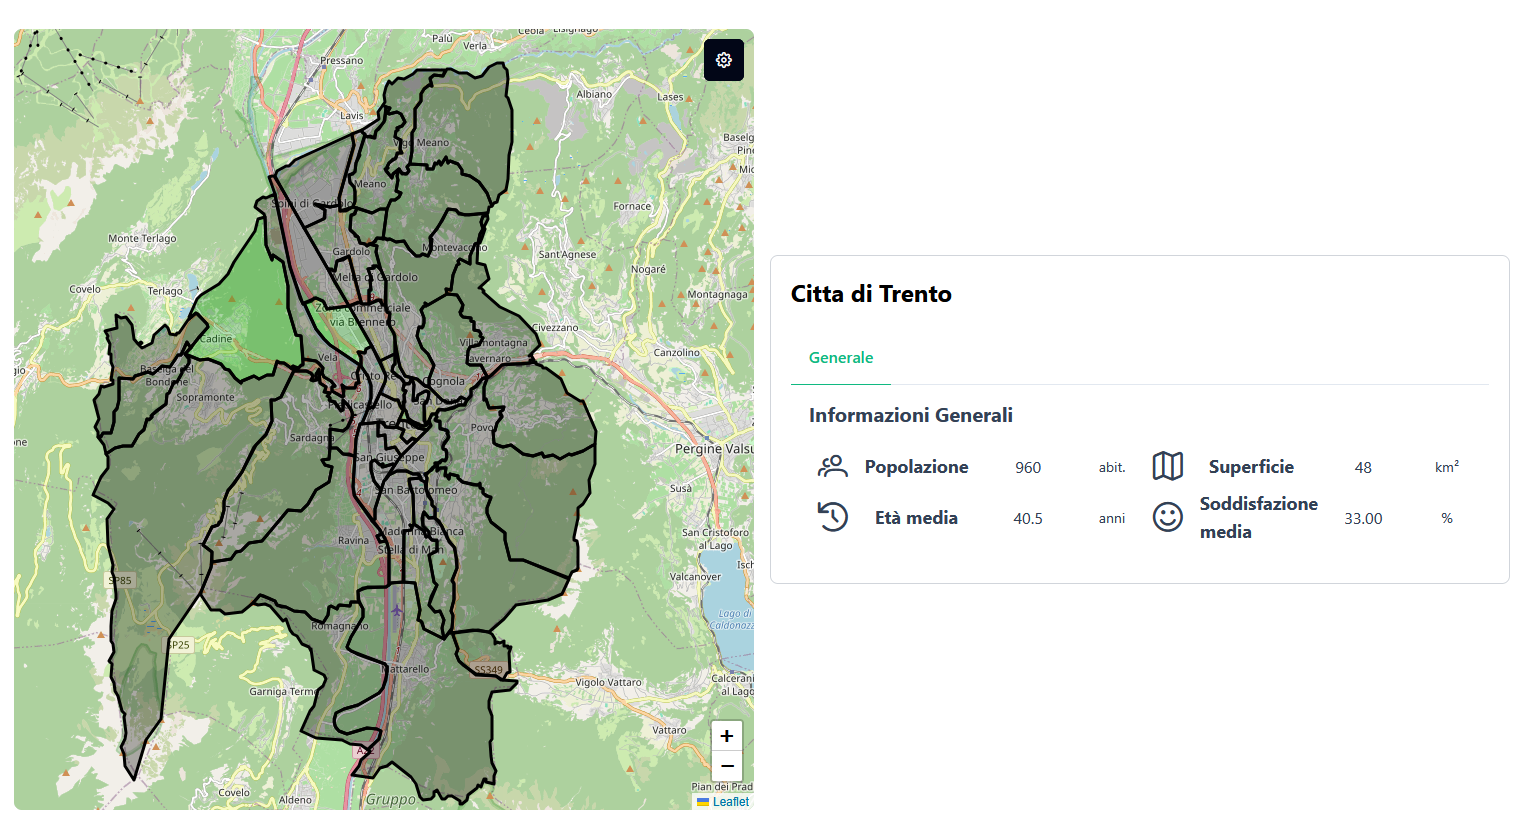
\includegraphics[width=0.8\textwidth]{frontend/home_analista.png}
        \caption{\textit{Home Page} per utenti con ruolo ``analista''}
        \label{fig:frontend-analista}
    \end{figure}
    Possiamo notare dalla Figura \Ref{fig:frontend-analista} come l'interfaccia grafica si sia differenziata rispetto alla Figura \Ref{fig:frontend-home}. Possiamo notare come le informazioni generali del comune siano comunque visibili ma sono raggruppate, non cambia molto infatti dalla \textit{homepage} delle altre tipologie di utenti. 
    \subsubsection{Selezione di un ``quartiere''/``circoscrizione'' - analista}
        \begin{figure}[H]
            \centering
            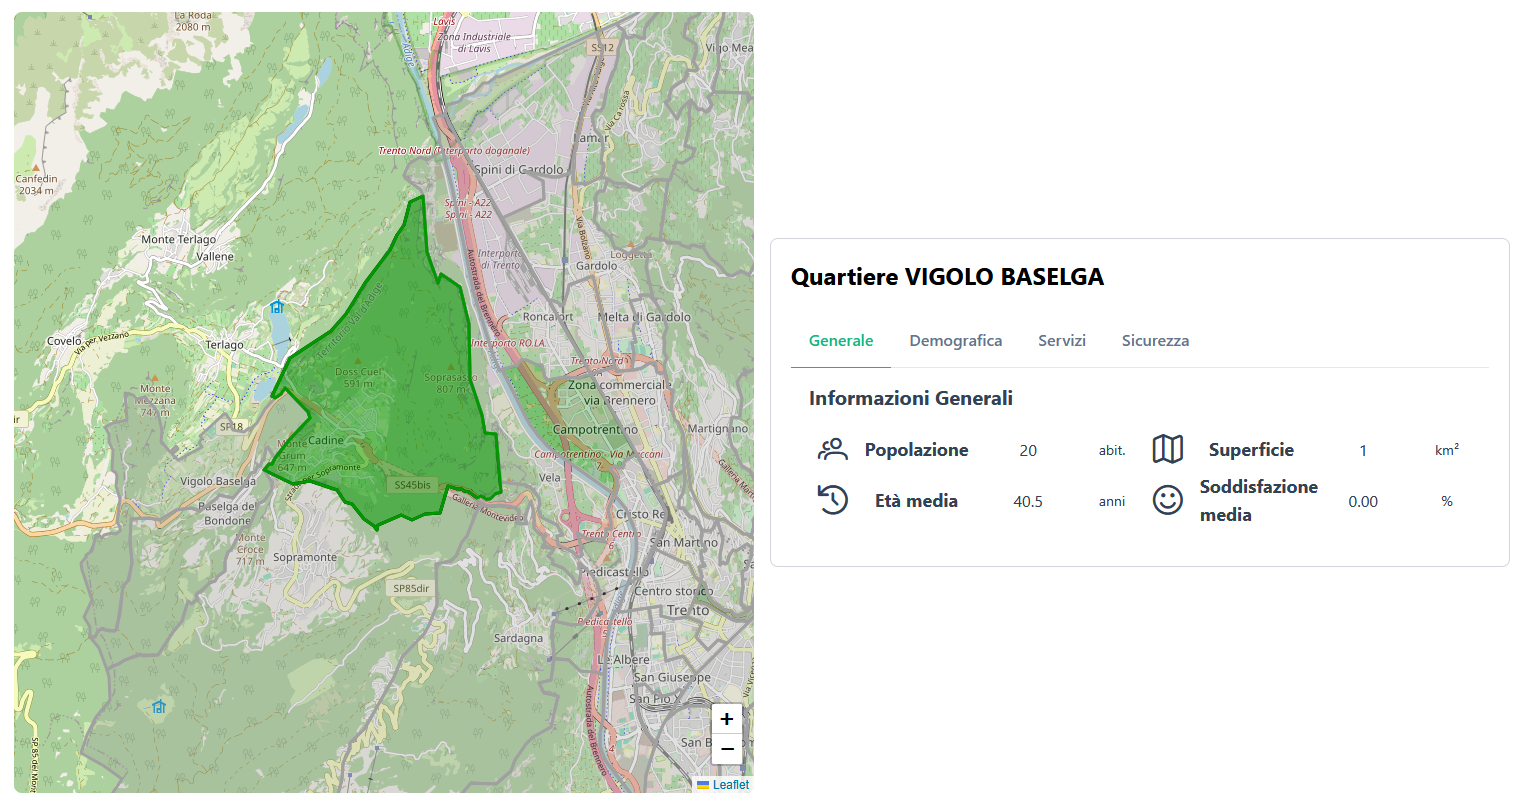
\includegraphics[width=0.8\textwidth]{frontend/alaisi_selezionato.png}
            \caption{Selezione di un ``quartiere''/``circoscrizione'' per utenti con ruolo ``analista''}
            \label{fig:frontend-analista-quartiere}
        \end{figure}
        Notiamo dalla Figura \Ref{fig:frontend-analista-quartiere} come la selezione di un ``quartiere'' o ``circoscrizione'' avvenga tramite un click sulla mappa come nel caso degli altri utenti. Una volta selezionato un ``quartiere'' o ``circoscrizione'' verranno visualizzati oltre alle informazioni generali del ``quartiere'' o della ``circoscrizione'' anche altri indicatori accessibili tramite le diverse pagine del menù posizionato sulla destra della mappa.\newline
        Si possa notare come questa visualizzazione sia una estensione della visualizzazione per gli altri utenti, dunque tutte le funzionalità e le azioni che il sistema compie alla selezione/deselezione sono le stesse.
    \subsubsection{Dettaglio menù impostazioni}
        \begin{figure}[H]
            \centering
            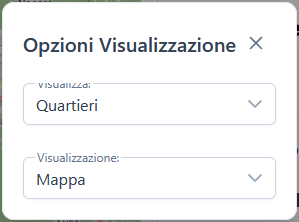
\includegraphics[width=0.3\textwidth]{frontend/opzioni_analista.png}
            \caption{Menù impostazioni per utenti con ruolo ``analista''}
            \label{fig:frontend-settings-analista}
        \end{figure}
        Il menù delle impostazioni per gli utenti con ruolo ``analista'' estende le funzionalità del menù per tutti gli altri utenti della figura \Ref{fig:frontend-settings}. In particolare, oltre alla possibilità di passare da una visualizzazione dei dati per quartieri ad una per circoscrizioni e viceversa, è possibile passare dalla visualizzazione di questi da una visualizzazione in ``mappa'' ad una in ``tabella''. Questo permette agli utenti con ruolo ``analista'' di avere una visione più dettagliata dei dati.
    \subsubsection{Visualizzazione dati in ``tabella''}
        \begin{figure}[H]
            \centering
            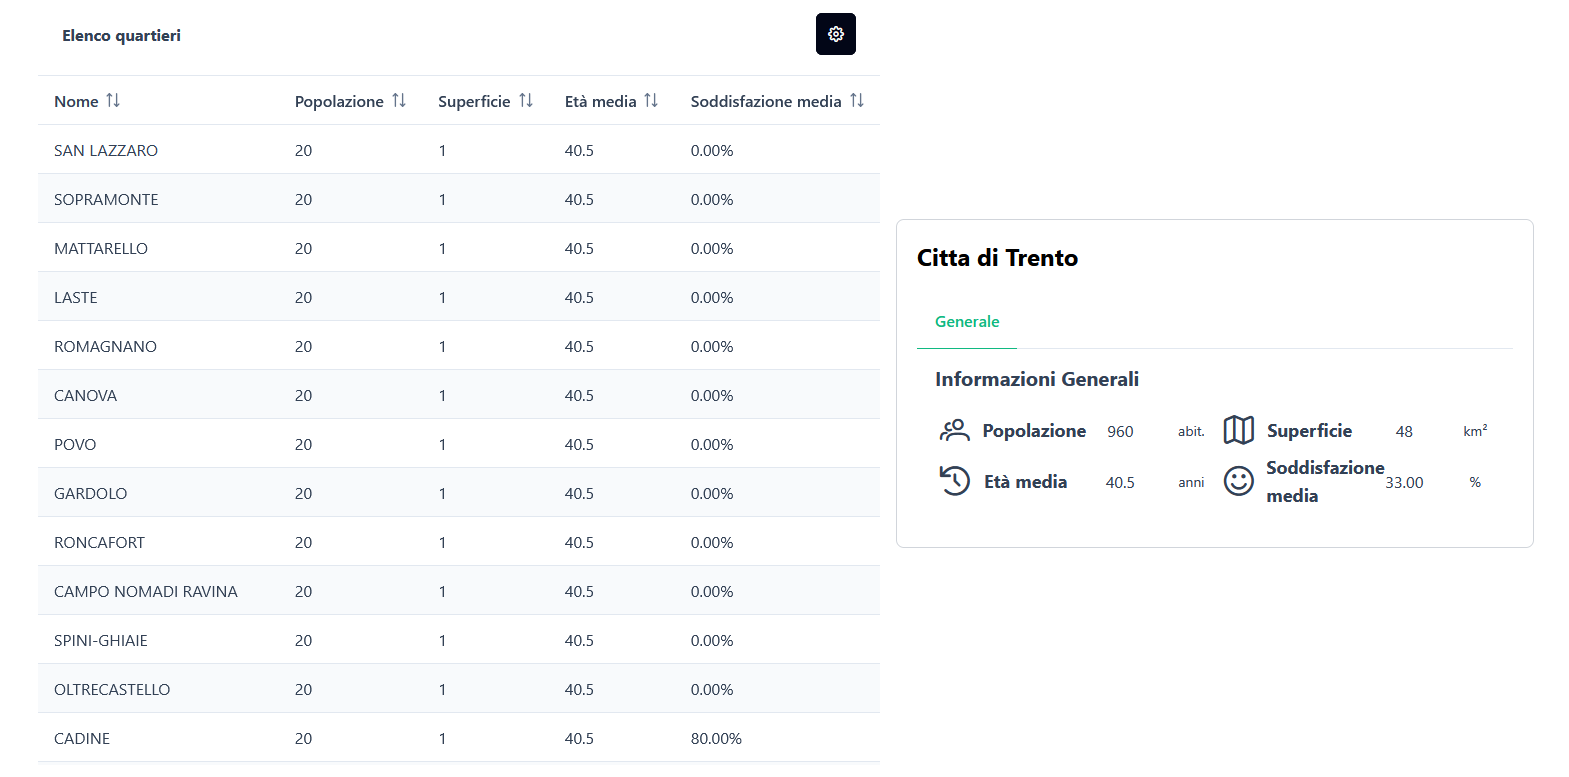
\includegraphics[width=0.8\textwidth]{frontend/home_analista_tabella.png}
            \caption{Visualizzazione dati in ``tabella''}
            \label{fig:frontend-analista-tabella}
        \end{figure}
        Nella Figura \Ref{fig:frontend-analista-tabella} è possibile vedere la visualizzazione dei dati in ``tabella'' per gli utenti con ruolo ``analista''. Questa visualizzazione permette di avere una visione, ordinabile per le colonne presenti, dei dati relativi ai ``quartieri'' o alle ``circoscrizioni''. Da questa visualizzazione è possibile selezionare un ``quartiere'' o una ``circoscrizione'' premendo sulla riga corrispondente. 
    \subsubsection{``Quartiere''/``circoscrizione'' selezionata in visualizzazione tabella}
        \begin{figure}[H]
            \centering
            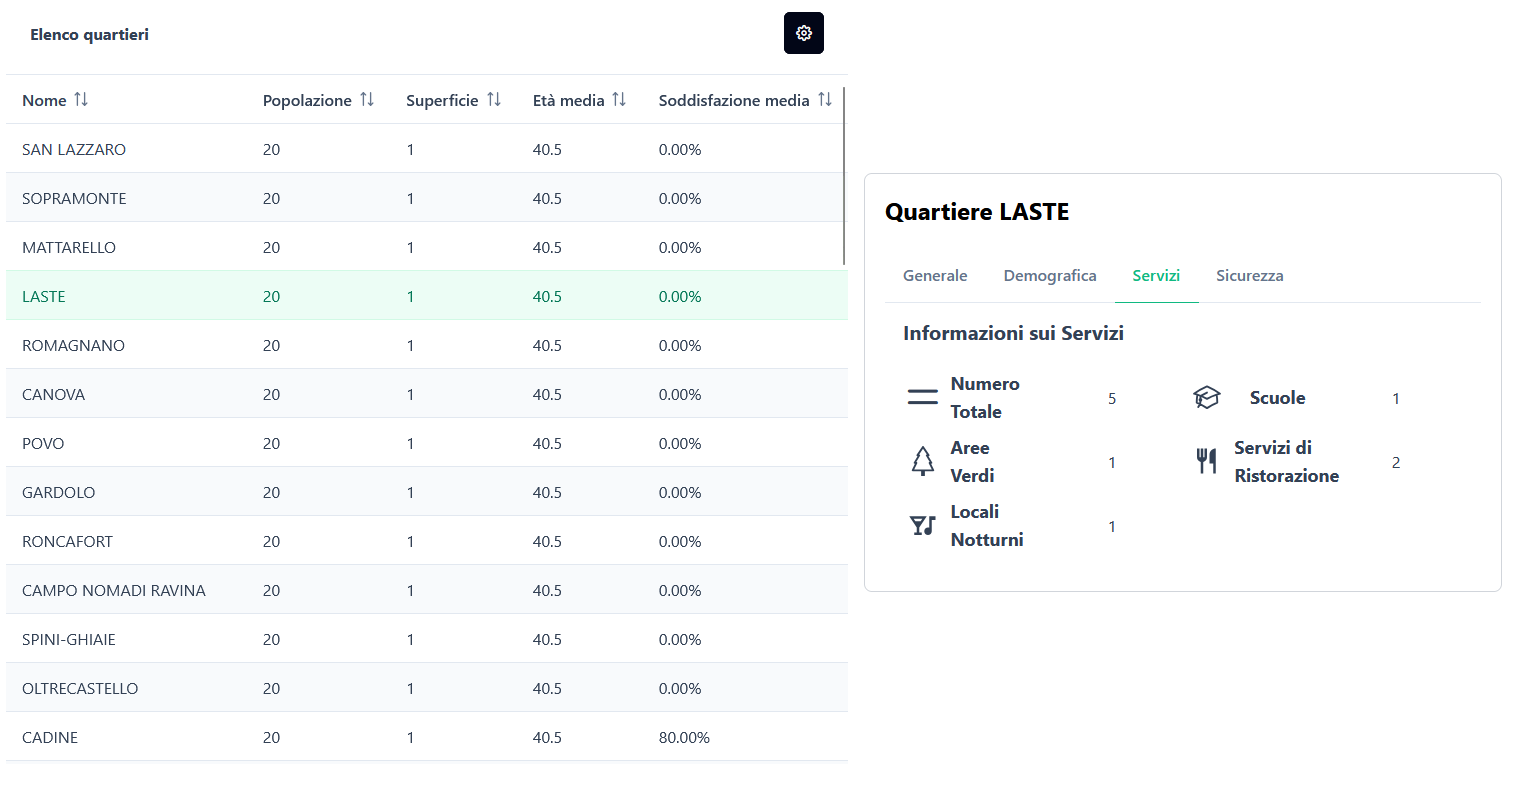
\includegraphics[width=0.8\textwidth]{frontend/alaisi_selezionato_tabella.png}
            \caption{``Quartiere''/``circoscrizione'' selezionata in visualizzazione tabella}
            \label{fig:frontend-analista-tabella-selezionato}
        \end{figure}
        La figura \Ref{fig:frontend-analista-tabella-selezionato} mostra come si presenta la visualizzazione di un ``quartiere'' o una ``circoscrizione'' selezionata in visualizzazione tabella. Questa situazione è una unione della selezione nel caso della figura \Ref{fig:frontend-analista-quartiere} e della visualizzazione in tabella della figura \Ref{fig:frontend-analista-tabella}. Da questa visualizzazione è possibile tornare alla visualizzazione dei dati della città selezionando il ``quartiere'' o la ``circoscrizione'' selezionata oppure è possibile cambiare ``quartiere'' o ``circoscrizione'' selezionando un altro ``quartiere'' o ``circoscrizione'' dalla tabella, in questo caso la riga selezionata verrà evidenziata ed i dati relativi al ``quartiere'' o alla ``circoscrizione'' selezionata verranno visualizzati.
\section{funzionalità Sondaggista}